\newcommand{\racetrack}[6]{%
  % (#1,#2) = centre
  % #3 = half total width
  % #4 = half total height
  % #5 = corner x-radius
  % #6 = corner y-radius
    ({#1 + #3}, {#2 - #4 + #6})
    arc[start angle=0, end angle=-90, x radius=#5, y radius=#6]
    -- ({#1 - #3 + #5}, {#2 - #4})
    arc[start angle=-90, end angle=-180, x radius=#5, y radius=#6]
    -- ({#1 - #3}, {#2 + #4 - #6})
    arc[start angle=180, end angle=90, x radius=#5, y radius=#6]
    -- ({#1 + #3 - #5}, {#2 + #4})
    arc[start angle=90, end angle=0, x radius=#5, y radius=#6]
    -- cycle
}
\newcommand{\ttlabel}[1]{\lstinline[basicstyle={\ttfamily\footnotesize}]{#1}}

\chapter{Aperture Modelling and Calculation}

\section{Overview and definitions}

\subsection{Aperture model}

The aperture module in \lstinline|xtrack/aperture| provides a geometric model of machine acceptance along an accelerator and tools to compare this acceptance with a beam envelope derived from Twiss data and a halo prescription.
The model is built from:
\begin{itemize}
    \item logical \emph{profile} shapes such as ellipses, rectangles, racetracks, etc., with associated tolerances;
    \item placements of these profiles inside a model of a \emph{pipe} section, which can be either straight or curved (an arc segment);
    \item placements of pipes, \emph{pipe positions}, along the survey of the machine.
\end{itemize}
When placing a profile in a pipe, or the pipe in the survey, transformations can be given.
In particular, the aperture model stores:
\begin{itemize}
	\item $(\Delta x, \Delta y, \Delta s, \phi, \theta, \psi)$ for each profile position within the pipe, where $\Delta s$ is the shift along the possibly curved frame of the pipe, and where the angles follow the usual conventions (see Chapter~\ref{chapter:misalignments} on misalignments);
	\item a $4 \times 4$ homogeneous transformation matrix for each pipe position, which specifies the placement of the pipe instance relative to the relevant survey reference point in the survey reference frame $(X, Y, Z)$.
\end{itemize}

\subsection{Aperture bounds}

Once a model is defined, the first step necessary before any aperture-related query is a pre-computation of so-called \emph{aperture bounds}.
This is a database associating every \emph{installed aperture} (a concrete instance of a profile in the model, i.e.~a particular \emph{profile position} within a pipe installed at a particular \emph{pipe position} in the line) with its location along the survey.
For every installed profile the survey $s$ positions spanning it are computed and memorised; this is illustrated in Figure~\ref{fig:aperture-bounds}.
For the common case of an aperture $i$ orthogonal to the survey, the bound will simply be $\{s_i\}$.
Aperture bounds are used for checking the validity of the model as well as for aperture interpolation.

\begin{figure}
	\centering
	\begin{tikzpicture}
		\draw[black, thick] (0, 0) arc (90:120:5);
		\draw[black, thick, ->] (0, 0) arc (90:60:5) node[below right] {$\hat{s}$};
		\draw[black, thick] (-0.3, -1.2) -- (0.3, 1.2);
		
		\draw[black, dashed] (-0.3, -1.2) -- ($(-0.3, -1.2)+(95:1.2)$);
		\draw[black, dashed] (0.3, 1.2) -- ($(0.3, 1.2)+(87:-1.2)$);
		
		\fill[black] (0, 0) circle (0.05) node[above left=0.3mm and -1.3mm] {$s_i$};
		\fill[black] ($(-0.3, -1.2)+(95:1.2)$) circle (0.05) node[below left=1.5mm and -1mm] {$s_{\textrm{start},i}$};
		\fill[black] ($(0.3, 1.2)+(87:-1.2)$) circle (0.05) node[below right=1mm and -1mm] {$s_{\textrm{end},i}$};
	\end{tikzpicture}
	\caption{Visualisation of an aperture bound for some installed aperture $i$.}\label{fig:aperture-bounds}
\end{figure}

\subsection{Profile shapes}

Each profile shape is converted once to a closed polygon with a fixed number of points.
This is done by sampling uniformly along the path length.
This gives a common polygon representation for all subsequent operations such as interpolation, ray intersection, and point-in-polygon checks.

\noindent
\begin{minipage}[c]{0.42\textwidth}
	\centering
	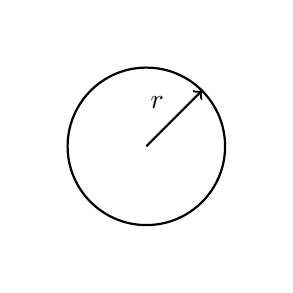
\begin{tikzpicture}
		\draw[white] (-1.5, -1.5) grid (1.5, 1.5);
		\draw[black, thick] (0, 0) circle (1);
		\draw[black, thick, ->] (0, 0) -- node[above left] {$r$} ({cos(45)}, {sin(45)});
	\end{tikzpicture}
\end{minipage}\hfill
\begin{minipage}[c]{0.54\textwidth}
\textbf{Circle.} Radius $r$.
\end{minipage}

\vspace{1em}
\noindent
\begin{minipage}[c]{0.42\textwidth}
	\centering
	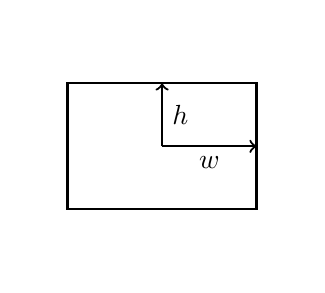
\begin{tikzpicture}
		\draw[white] (-1.7, -1.5) grid (1.7, 1.5);
		\draw[black, thick] (-1.2, -0.8) rectangle (1.2, 0.8);
		\draw[black, thick, ->] (0, 0) -- node[below] {$w$} (1.2, 0);
		\draw[black, thick, ->] (0, 0) -- node[right] {$h$} (0, 0.8);
	\end{tikzpicture}
\end{minipage}\hfill
\begin{minipage}[c]{0.54\textwidth}
\textbf{Rectangle.} Half-width $w$ and half-height $h$.
\end{minipage}

\vspace{1em}
\noindent
\begin{minipage}[c]{0.42\textwidth}
	\centering
	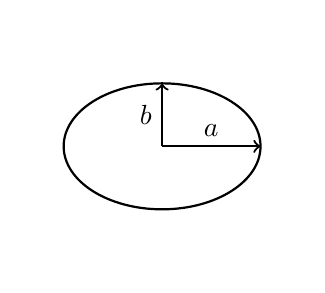
\begin{tikzpicture}
		\draw[white] (-1.7, -1.5) grid (1.7, 1.5);
		\draw[black, thick] (0, 0) ellipse (1.25 and 0.8);
		\draw[black, thick, ->] (0, 0) -- node[above] {$a$} (1.25, 0);
		\draw[black, thick, ->] (0, 0) -- node[left] {$b$} (0, 0.8);
	\end{tikzpicture}
\end{minipage}\hfill
\begin{minipage}[c]{0.54\textwidth}
\textbf{Ellipse.} Half-major axis $a$ and half-minor axis $b$.
\end{minipage}

\vspace{1em}
\noindent
\begin{minipage}[c]{0.42\textwidth}
	\centering
	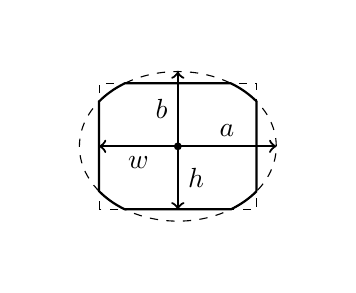
\begin{tikzpicture}
		\pgfmathsetmacro{\rw}{1.0}
		\pgfmathsetmacro{\rh}{0.8}
		\pgfmathsetmacro{\ea}{1.25}
		\pgfmathsetmacro{\eb}{0.95}
		\pgfmathsetmacro{\angA}{acos(\rw/\ea)}
		\pgfmathsetmacro{\angB}{asin(\rh/\eb)}
		\pgfmathsetmacro{\ix}{\ea*cos(\angB)}
		\pgfmathsetmacro{\iy}{\eb*sin(\angA)}
		\draw[white] (-1.9, -1.5) grid (1.9, 1.5);
		\draw[black, dashed] (-\rw, -\rh) rectangle (\rw, \rh);
		\draw[black, thick]
			(\rw, -\iy) -- (\rw, \iy)
			arc[start angle=\angA, end angle=\angB, x radius=\ea, y radius=\eb]
			-- (-\ix, \rh)
			arc[start angle=180-\angB, end angle=180-\angA, x radius=\ea, y radius=\eb]
			-- (-\rw, -\iy)
			arc[start angle=180+\angA, end angle=180+\angB, x radius=\ea, y radius=\eb]
			-- (\ix, -\rh)
			arc[start angle=360-\angB, end angle=360-\angA, x radius=\ea, y radius=\eb];
		\draw[black, dashed] (0, 0) ellipse [x radius=\ea, y radius=\eb];
		\fill[black] (0, 0) circle (0.05);
		\draw[black, thick, ->] (0, 0) -- node[below] {$w$} (-\rw, 0);
		\draw[black, thick, ->] (0, 0) -- node[right] {$h$} (0, -\rh);
		\draw[black, thick, ->] (0, 0) -- node[above] {$a$} (\ea, 0);
		\draw[black, thick, ->] (0, 0) -- node[left] {$b$} (0, \eb);
	\end{tikzpicture}
\end{minipage}\hfill
\begin{minipage}[c]{0.54\textwidth}
\textbf{Rectellipse.} Half-width $w$, half-height $h$, half-major axis $a$, and half-minor axis $b$.
\end{minipage}

\vspace{1em}
\noindent
\begin{minipage}[c]{0.42\textwidth}
	\centering
	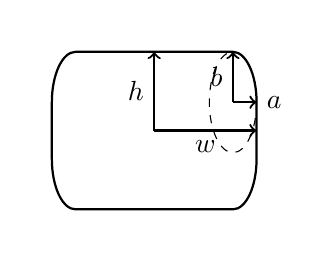
\begin{tikzpicture}
		\draw[white] (-1.6, -1.3) grid (1.6, 1.3);
		\draw[black, thick] \racetrack{0}{0}{1.3}{1}{0.3}{0.64};
		\draw[black, dashed] (1.0, 0.36) ellipse [x radius=0.3, y radius=0.64];
		\draw[black, thick, ->] (0, 0) -- node[below] {$w$} (1.3, 0);
		\draw[black, thick, ->] (0, 0) -- node[left] {$h$} (0, 1.0);
		\draw[black, thick, ->] (1.0, 0.36) -- (1.3, 0.36) node[right] {$a$};
		\draw[black, thick, ->] (1.0, 0.36) -- node[left] {$b$} (1.0, 1.0);
	\end{tikzpicture}
\end{minipage}\hfill
\begin{minipage}[c]{0.54\textwidth}
\textbf{Racetrack.} Half-width $w$, half-height $h$, and ellipse-corner half-axes $a$, $b$.
\end{minipage}

\vspace{1em}
\noindent
\begin{minipage}[c]{0.42\textwidth}
	\centering
	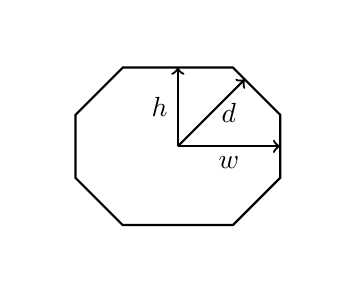
\begin{tikzpicture}
		\pgfmathsetmacro{\ow}{1.3}
		\pgfmathsetmacro{\oh}{1.0}
		\pgfmathsetmacro{\od}{1.7/sqrt(2)}
		\pgfmathsetmacro{\ox}{\od*sqrt(2)-\oh}
		\pgfmathsetmacro{\oy}{\od*sqrt(2)-\ow}
		\pgfmathsetmacro{\of}{\od/sqrt(2)}
		\draw[white] (-1.9, -1.5) grid (1.9, 1.5);
		\draw[black, thick]
			(-\ox, -\oh) -- (\ox, -\oh) -- (\ow, -\oy) -- (\ow, \oy) --
			(\ox, \oh) -- (-\ox, \oh) -- (-\ow, \oy) -- (-\ow, -\oy) -- cycle;
		\draw[black, thick, ->] (0, 0) -- node[below] {$w$} (\ow, 0);
		\draw[black, thick, ->] (0, 0) -- node[left] {$h$} (0, \oh);
		\draw[black, thick, ->] (0, 0) -- node[right] {$d$} (\of, \of);
	\end{tikzpicture}
\end{minipage}\hfill
\begin{minipage}[c]{0.54\textwidth}
\textbf{Octagon.} Half-width $w$, half-height $h$, and half-diagonal gap $d$.
\end{minipage}

\vspace{1em}
\noindent
\begin{minipage}[c]{0.42\textwidth}
	\centering
	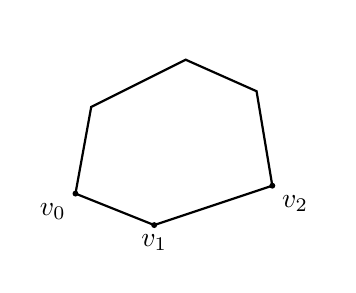
\begin{tikzpicture}
		\draw[white] (-1.9, -1.5) grid (1.9, 1.5);
		\draw[black, thick]
			(-1.3, -0.6) -- (-0.3, -1.0) -- (1.2, -0.5) -- (1.0, 0.7) --
			(0.1, 1.1) -- (-1.1, 0.5) -- cycle;
		\filldraw[black] (-1.3, -0.6) circle (0.03) node[below left] {$v_0$};
		\filldraw[black] (-0.3, -1.0) circle (0.03) node[below] {$v_1$};
		\filldraw[black] (1.2, -0.5) circle (0.03) node[below right] {$v_2$};
	\end{tikzpicture}
\end{minipage}\hfill
\begin{minipage}[c]{0.54\textwidth}
\textbf{Polygon.} Arbitrary polygon given by an ordered list of vertices $(v_0, v_1, \ldots) = ((x_0, y_0), (x_1, y_1), \ldots)$.
\end{minipage}

\subsection{Profiles}

A \emph{profile} is a shape together with three tolerances:
\begin{itemize}
    \item \lstinline|tol_r|: radial tolerance,
    \item \lstinline|tol_x|: horizontal tolerance,
    \item \lstinline|tol_y|: vertical tolerance.
\end{itemize}
These effectively form a tolerance racetrack with half-width of $\text{\lstinline|tol_x|} + \text{\lstinline|tol_r|}$, half-height $\text{\lstinline|tol_y|} + \text{\lstinline|tol_r|}$, and a circular radius of $\text{\lstinline|tol_r|}$.

%	\begin{tikzpicture}
%		\draw[white] (-2, 2) grid (2, 2);
%		\draw[black, thick]
%			(1.5, -0.5)
%			arc[start angle=0, end angle=-90, radius=0.5]
%			-- (-1.0, -1.0)
%			arc[start angle=-90, end angle=-180, radius=0.5]
%			-- (-1.5, 0.5)
%			arc[start angle=180, end angle=90, radius=0.5]
%			-- (1.0, 1.0)
%			arc[start angle=90, end angle=0, radius=0.5]
%			-- cycle;
%
%		\draw[black, dashed] (1, 0.5) -- (1, -0.5) -- (-1, -0.5) -- (-1, 0.5) -- cycle;
%
%		\draw[black, thick, ->] (0, 0) -- node[below] {$w$} (1.0, 0);
%		\draw[black, thick, ->] (0, 0) -- node[left] {$h$} (0, 0.5);
%		\draw[black, thick, ->] (1.0, 0.5) -- (1.5, 0.5) node[right] {$a$};
%		\draw[black, thick, ->] (1.0, 0.5) -- node[left] {$b$} (1.0, 1.0);
%	\end{tikzpicture}

\subsection{Beam envelope}\label{subsec:apertures-beam-envelope}

The beam-envelope calculation uses:
\begin{itemize}
    \item local optics and closed orbit values,
    \item beam and tolerance parameters specified by the user,
    \item aperture tolerances of the local profile.
\end{itemize}
In particular, \lstinline{halo_params} define the following beam parameters:
\begin{itemize}
	\item \lstinline{emitx_norm} ($\varepsilon_{x,\mathrm{n}}$) and \lstinline{emity_norm} ($\varepsilon_{y,\mathrm{n}}$) -- normalised emmittances (unitless),
    \item \lstinline{delta_rms} ($\delta_\mathrm{rms}$) -- root-mean-square relative momentum spread (unitless),
    \item \lstinline{tol_co} ($r_\mathrm{co}$) -- closed orbit error (in metres),
    \item \lstinline{tol_disp} ($f_D$) -- dispersion tolerance scaling factor (unitless),
    \item \lstinline{tol_disp_ref} ($D_\mathrm{ref}$) -- reference dispersion error (in metres),
    \item \lstinline{tol_disp_ref_beta} ($\beta_{D,\mathrm{ref}}$) -- reference beta for dispersion scaling (in metres),
    \item \lstinline{tol_beta_beating} ($f_\beta$) -- beta beating tolerance scaling factor (unitless).
    \item $h_x := \frac{\text{\lstinline{halo_x}}}{\text{\lstinline{halo_primary}}}$, $h_y := \frac{\text{\lstinline{halo_y}}}{\text{\lstinline{halo_primary}}}$, and $h_r := \frac{\text{\lstinline{halo_r}}}{\text{\lstinline{halo_primary}}}$ -- reference horizontal, vertical, and radial size of the beam in the units of betatron sigma.
\end{itemize}
The optical beam sizes for a one-betatron sigma beam are given by
\[
\sigma_x = \sqrt{\frac{\varepsilon_{x,\mathrm{n}}}{\gamma_r\beta_r}\beta_x} \cdot f_\beta,
\qquad
\sigma_y = \sqrt{\frac{\varepsilon_{y,\mathrm{n}}}{\gamma_r\beta_r}\beta_y} \cdot f_\beta.
\]
We model the beam as a racetrack of shape determined by the parameters $h_x$, $h_y$, and $h_r$.
To obtain the modelled $n$-sigma beam envelope in metres, the racetrack defined by the above parameters is scaled by $(n\sigma_x, n\sigma_y)$:
\[
	n \cdot \text{\lstinline{beam_racetrack}} :=
	n
	\begin{bmatrix}
	  \sigma_x \\
	  \sigma_y 
	\end{bmatrix}
	\cdot
	\begin{tikzpicture}[baseline={(0, -1mm)}]
		\draw[white] (-1.6, -1.2) grid (1.6, 1.2);
		\draw[black, thick] \racetrack{0}{0}{1.5}{1}{0.5}{0.5};

		%\draw[black, dashed] (1, 0.5) circle (0.5);
		\draw[black, dashed] (1, 0.5) -- (1, -0.5) -- (-1, -0.5) -- (-1, 0.5) -- cycle;

		\draw[black, thick, ->] (0, 0) -- node[below] {$h_x$} (1.5, 0);
		\draw[black, thick, ->] (0, 0) -- node[left] {$h_y$} (0, 1);

		\draw[black, thick, ->] (0, 0) -- node[above] {$h_r$} ($(1.0, 0.5) + (26.6:0.5)$);
	\end{tikzpicture}
\]
Separately, we can build a tolerance racetrack which includes:
\begin{itemize}
    \item the individual aperture tolerances \lstinline|tol_x|, \lstinline|tol_y|, \lstinline|tol_r|,
    \item uncorrelated (also referred to as \emph{spurious}) dispersion orbit shift:
    \[
		\Delta x_{D,\beta} := f_\beta \cdot f_D \cdot D_\mathrm{ref} \cdot \sqrt{\frac{\beta_x}{\beta_{D,\mathrm{ref}}}} \cdot \delta_\mathrm{rms},
		\qquad
		\Delta y_{D,\beta} := f_\beta \cdot f_D \cdot D_\mathrm{ref} \cdot \sqrt{\frac{\beta_y}{\beta_{D,\mathrm{ref}}}} \cdot \delta_\mathrm{rms},
	\]
    \item and the closed-orbit tolerance $r_\mathrm{co}$.
\end{itemize}
This racetrack can be visualised as (where $+$ denotes convolution/Minkowski sum):
\[
	\text{\lstinline{halo_racetrack}} :=
	\begin{tikzpicture}[baseline={(0, -1mm)}]
		\draw[black, thick] \racetrack{0}{0}{1.2}{1}{0.5}{0.5};

		%\draw[black, dashed] (1, 0.5) circle (0.5);
		\draw[black, dashed] (0.7, 0.5) -- (0.7, -0.5) -- (-0.7, -0.5) -- (-0.7, 0.5) -- cycle;

		\draw[black, thick, ->] (0, 0) -- node[below] {\ttlabel{tol_x}} (0.7, 0);
		\draw[black, thick, ->] (0, 0) -- node[left] {\ttlabel{tol_y}} (0, 0.5);

		\draw[black, thick, ->] (0.7, 0.5) -- node[left] {\ttlabel{tol_r}} ($(0.7, 0.5) + (45:0.5)$);
	\end{tikzpicture}
	\;+\;
	\begin{tikzpicture}[baseline={(0, -1mm)}]
		\draw[black, thick] (0, 0) ellipse (1.25 and 0.8);
		\draw[black, thick, ->] (0, 0) -- node[below left = 0 and -4mm] {$\Delta x_{D,\beta}$} (1.25, 0);
		\draw[black, thick, ->] (0, 0) -- node[below left = -2mm and -1mm] {$\Delta y_{D,\beta}$} (0, 0.8);
	\end{tikzpicture}
	\;+\;
		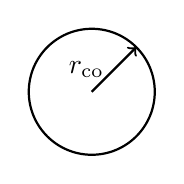
\begin{tikzpicture}[baseline={(0, -1mm)}]
		\draw[black, thick] (0, 0) circle (0.8);
		\draw[black, thick, ->] (0, 0) -- node[left] {$r_\mathrm{co}$} (45:0.8);
	\end{tikzpicture}
\]
Since racetracks are closed under convolution, we can represent our beam envelope at $n$-sigmas (without including correlated dispersion orbit shift yet) as:
\[
	\text{\lstinline{envelope}}(n) := \text{\lstinline{halo_racetrack}} + n \cdot \text{\lstinline{beam_racetrack}}.
\]
Depending on the algorithm this representation will be converted to a polygon (beam envelope generation functions, bisection method for computing the max aperture sigma) or will be used directly for analytic calculations.

In aperture calculations we must further include the orbit shift error induced by correlated dispersion, also referred to as \emph{model} dispersion.
In the case of converting to a polygon, we can further include the  in the resulting shape by `stretching' it.
We can convolve $\text{\lstinline{envelope}}(n)$ with the line segment segment $[-\mathbf{v}_{D,\mathrm{model}}, \mathbf{v}_{D,\mathrm{model}}]$, where
\[
	\mathbf{v}_{D,\mathrm{model}} := \begin{bmatrix}
	  D_x \delta_\mathrm{rms} \\
	  D_y \delta_\mathrm{rms}
	\end{bmatrix},
\]
to obtain an $n$-sigma beam envelope including the error related to correlated dispersion, as well us uncorrelated dispersion error, aperture tolerance, and the close orbit tolerance errors.
In case of analytic methods, we will usually separately consider two envelopes shifted by $\pm\mathbf{v}_{D,\mathrm{model}}$ instead.

\section{Algorithms}

\subsection{Aperture bounds}

For any installed profile let (where by pose we mean the position and orientation)
\begin{itemize}
	\item $M_S$ be the pose of the pipe's survey reference point in the survey frame,
	\item $M_T$ be the pose of the pipe's origin $(x, y, s) = (0, 0, 0)$ relative to the survey reference point,
	\item $M_P$ be the pose representing the installed profile's position within the pipe frame.
\end{itemize}
Then, the $M_{P,\mathrm{world}} = M_S \, M_T \, M_P$ represents the position and orientation of the installed profile in world coordinates (survey frame).
In order to calculate the locations of the installed profiles in the survey frame, we perform the intersection of the profile plane (local $s = 0$ in the $M_{P,\mathrm{world}}$ frame) with the survey curve.
Each segment of the survey is defined as either a line segment or an arc segment, and we work our way outwards from the survey reference point testing for intersection, until a valid $s$ is found.
The bounds $s_\mathrm{start}$ and $s_\mathrm{end}$ are computed by projecting each 3D polygon point of a given installed profile onto the survey curve and taking the minimum, and the maximum values.

As mentioned in this chapter's introduction, aperture bounds are used for checking the validity of the model as well as for aperture interpolation.
Since $s_i$ (for some aperture $i$) is calculated as an aperture-plane--survey-curve intersection, and $s_{\textrm{min},i}$ and $s_{\textrm{max},i}$ are aperture extremes projected onto the survey curve, if for any aperture $s_i \not\in [s_{\textrm{min},i}, s_{\textrm{max},i}]$, we know the model is invalid as the aperture sits outside of the machine.
Additionally, we disallow models with overlapping aperture bounds.

\subsection{Cross section interpolation}

The module is capable of computing the aperture polygons in the plane orthogonal to an arbitrary $s$-position along the survey.
Aperture bounds are used to find the correct installed apertures that need to be interpolated.
If the $s$ position for interpolation sits outside of any bounds, we interpolate the profiles on either side of $s$.
However, if the $s$ position sits within a bound of some aperture $i$, we need to partly interpolate $i - 1$ with $i$, and partly interpolate $i$ with $i + 1$.
This is illustrated in Figures~\ref{fig:aperture-interpolation-simple} and~\ref{fig:aperture-interpolation-both-sides}.
Aperture tolerances are also interpolated from the neighbouring profiles.

\begin{figure}
	\centering
	\begin{tikzpicture}
		\draw[black, thick, ->] (-3, 0) -- (3.5, 0) node[below right] {$\hat{s}$};

		\draw[black, thick] (-1.3, -1.2) -- (-0.7, 1.2);
		\draw[black, dashed] (-1.3, -1.2) -- (-1.3, 0);
		\draw[black, dashed] (-0.7, 1.2) -- (-0.7, 0);

		\draw[black, thick] (1.9, -1.5) -- (1.3, 1.5);		
		\draw[black, dashed] (1.9, -1.5) -- (1.9, 0);
		\draw[black, dashed] (1.3, 1.5) -- (1.3, 0);
		
		\draw[red, thick] (0.3, 1.35) -- (0.3, -1.35);
		
		\fill[black] (0.3, 0) circle (0.05) node[below right] {$s_q$};
		\draw[black, dashed] (0.3, -2) -- (0.3, 2);
		\draw[black]  (0.3, 0.2) -- (0.5, 0.2) -- (0.5, 0);

		\draw[black, dotted] (-0.7, 1.2) -- (1.3, 1.5);
		\fill[black] (0.3, 1.35) circle (0.05) node[above left] {$P$};

		\draw[black, dotted] (-1.3, -1.2) -- (1.9, -1.5);
		\fill[black] (0.3, -1.35) circle (0.05) node [below left] {$Q$};
	\end{tikzpicture}
	\caption{Visualisation of aperture interpolation at some $s_q$ outside of any aperture bounds. The points $P$ and $Q$ are obtained by interpolating corresponding vertices of profiles on either side of $s_q$.}\label{fig:aperture-interpolation-simple}
\end{figure}

\begin{figure}
	\centering
	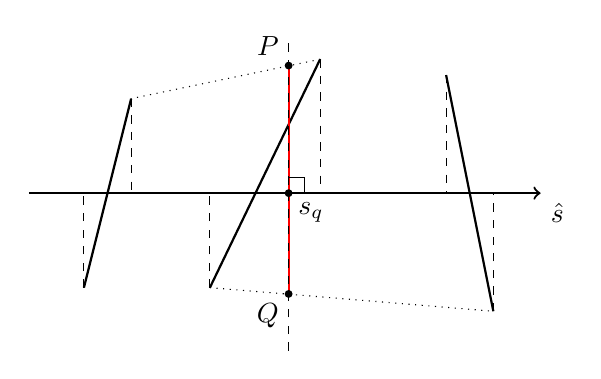
\begin{tikzpicture}
		\draw[black, thick, ->] (-3, 0) -- (3.5, 0) node[below right] {$\hat{s}$};

		\draw[black, thick] (-0.7, -1.2) -- (0.7, 1.7);
		\draw[black, dashed] (-0.7, -1.2) -- (-0.7, 0);
		\draw[black, dashed] (0.7, 1.7) -- (0.7, 0);
		%\fill[black] (-0.12, 0) circle (0.05);
		
		\draw[black, thick] (-2.3, -1.2) -- (-1.7, 1.2);
		\draw[black, dashed] (-2.3, -1.2) -- (-2.3, 0);
		\draw[black, dashed] (-1.7, 1.2) -- (-1.7, 0);
		
		\draw[black, thick] (2.9, -1.5) -- (2.3, 1.5);
		\draw[black, dashed] (2.9, -1.5) -- (2.9, 0);
		\draw[black, dashed] (2.3, 1.5) -- (2.3, 0);
		
		\draw[red, thick] (0.3, 1.62) -- (0.3, -1.28);
		
		\fill[black] (0.3, 0) circle (0.05) node[below right] {$s_q$};
		\draw[black, dashed] (0.3, -2) -- (0.3, 2);
		\draw[black]  (0.3, 0.2) -- (0.5, 0.2) -- (0.5, 0);
		
		\draw[black, dotted] (0.7, 1.7) -- (-1.7, 1.2);
		\fill[black] (0.3, 1.62) circle (0.05) node[above left] {$P$};
		
		\draw[black, dotted] (-0.7, -1.2) -- (2.9, -1.5);
		\fill[black] (0.3, -1.28) circle (0.05) node[below left] {$Q$};
	\end{tikzpicture}
	\caption{If $s_q$ falls within bounds of an installed aperture, some of the vertices of the new cross section need to be interpolated with the aperture to the left, such as point $P$, while other ones with the aperture to the right, such as point $Q$.}\label{fig:aperture-interpolation-both-sides}
\end{figure}

For a query at longitudinal position $s$, interpolation is performed in the cross-section plane defined by the resampled survey pose at that $s$; in practice the plane is transformed into the pipe frame (specifically the pipe containing $s$, or if $s$ falls in a gap, the earliest preceding one in $s$) and the neighbouring installed profiles and the target plane are all brought to this frame.
This is done to limit numerical noise that might otherwise be present when mixing small local quantities with world coordinates.

The profiles are uniformly discretised into the same number of points and the first step before actual interpolation is determining point correspondence between the profiles.
This is done after projecting the neighbouring polygons into the target cross-section plane: a cyclic shift is chosen so that the projected point ordering minimises the sum of distances between corresponding vertices.
Interpolation then proceeds by connecting corresponding 3D vertices from the two neighbouring installed profiles and intersecting those line segments with the target plane.

The procedure is more complex for curved pipes, where the following approximation is employed.
Note that, for a curved pipe, $M_P$ already includes the motion along the curved reference axis, i.e. the profile is first advanced by the pipe curvature to its local $s$-location and then given its local offsets/rotations.
During interpolation, the segment-plane intersection is handled after `straightening' the curvilinear frame.
Given a Cartesian frame and a curvilinear frame with curvature $h$ (or equivalently radius $R = h^{-1}$) whose origins coincide, a Cartesian point can be transformed into a curvilinear point as follows:
\[
	\begin{bmatrix} x \\ y \\ s \end{bmatrix} =
	\begin{bmatrix}
		\mathrm{sgn}(h) \sqrt{(X+R)^2+Z^2}-R \\
		Y \\
		R \cdot \mathrm{atan}_2\left(\mathrm{sgn}(h) Z,\, \mathrm{sgn}(h)(X + R)\right)
	\end{bmatrix}.
\]
We can transform a plane, which is represented as a (Cartesian) normal $(v_X, v_Y, v_Z)$ attached to a (curvilinear) point $(x, y, s)$, like so:
\[
	\begin{bmatrix} v_x \\ v_y \\ v_s \end{bmatrix} =
	\begin{bmatrix}
		\cos(hs) & 0 & \sin(hs) \\
		0 & 1 & 0 \\
		-\frac{\sin(hs)}{1+h x} & 0 & \frac{\cos(hs)}{1+h x}
	\end{bmatrix}
	\begin{bmatrix} v_X \\ v_Y \\ v_Z \end{bmatrix}.
\]
Once the two polygon points together with the plane's point and normal are transformed, we can perform the intersection in the `straightened' frame with the usual algorithm.
The resulting point can be converted back to the Cartesian plane with:
\[
	\begin{bmatrix} X \\ Y \\ Z \end{bmatrix} =
	\begin{bmatrix}
        (R + x) \cos(h s) - R \\
        y \\
        (R + x) \sin(h s)
    \end{bmatrix}.
\]

\subsection{Maximum beam sigma}

There are three methods currently implemented for computing the maximum number of sigmas for which the beam fits in a given cross section; this quantity is ofter referred to as $n_1$:
\begin{equation}\label{eq:apertures-n1}
	n_1 := \sup \left\{ n \;|\; \text{\lstinline{total_envelope}}(n) \subset \text{\lstinline{cross_section}} \right\}.
\end{equation}
The \lstinline{total_envelope} corresponds to \lstinline{envelope} with the correlated dispersion error applied; the precise method of the application of this error, and the computation of $n_1$ is what distinguishes the three different algorithms implemented in Xtrack.
These algorithms are described below.

\subsubsection{`Bisection' method}

The \emph{bisection} method computes $n_1$ as the largest beam scale factor for which the full beam envelope polygon still fits inside the interpolated aperture polygon.
In particular, the beam envelope is discretised to a polygon which includes the dispersive orbit error as a `stretch' described in Section~\ref{subsec:apertures-beam-envelope}, and visualised in Fig.~\ref{fig:aperture-bisection}.
At each $s$ a trial envelope is repeatedly built, the algorithm checks polygon containment, and bisects until the limiting value is found.
It is the most direct geometric implementation of Eq.~\ref{eq:apertures-n1}, but also the most expensive at  $O(EAK)$, where $E$ is the number of envelope points,
              $A$ is the number of aperture points, and $K = \log_2(\frac{\text{search space}}{\text{search tolerance}})$ is the number of bisection steps, currently $K \leq 25$.

\begin{figure}
	\centering
	\begin{tikzpicture}
		\draw[white] (-4, -3) grid (4, 3);
		
		\draw[black, dashed] \racetrack{0}{0}{1.5}{1}{0.5}{0.5};
		\draw[black, dashed] \racetrack{1.35}{0.85}{0.8}{1.2}{0.8}{1.2};
		\draw[black, dashed] \racetrack{0}{0}{2.3}{2.2}{1.3}{1.7};
		
		\draw[black] (-0.07, -0.07) -- (0.07, 0.07); \draw[black] (0.07, -0.07) -- (-0.07, 0.07);
		\draw[black, ->] ($(-1, 0.5) + (-220:1.3 and 1.7)$) -- ++(-0.5, 0.5) node[left] {\footnotesize$\mathbf{v}_{D,\text{model}}$};
		\draw[black, ->] ($(1, -0.5) - (-220:1.3 and 1.7)$) -- ++(0.5, -0.5) node[right] {\footnotesize$-\mathbf{v}_{D,\text{model}}$};
		
		\draw[black, thick] ({0 + 2.3 + 0.5}, {0 - 2.2 + 1.7 - 0.5})
		    arc[start angle=0, end angle=-90, x radius=1.3, y radius=1.7]
		    -- ({0 - 2.3 + 1.3 + 0.5}, {0 - 2.2 - 0.5})
		    arc[start angle=-90, end angle=-130, x radius=1.3, y radius=1.7]
		    -- ++(-1, 1)
		    arc[start angle=-130, end angle=-180, x radius=1.3, y radius=1.7]
		    -- ({0 - 2.3 - 0.5}, {0 + 2.2 - 1.7 + 0.5})
		    arc[start angle=180, end angle=90, x radius=1.3, y radius=1.7]
		    -- ({0 + 2.3 - 1.3 - 0.5}, {0 + 2.2 + 0.5})
		    arc[start angle=90, end angle=50, x radius=1.3, y radius=1.7]
		    -- ++(1, -1)
		    arc[start angle=50, end angle=0, x radius=1.3, y radius=1.7]
		    -- cycle;
		
		\draw (0, -1) node[below] {\footnotesize\lstinline{halo_rt}};
		\fill[black] (1.35, 0.85) circle (0.05);
		\draw (1.35, {0.85 - 1.2}) node[below] {\footnotesize$n \, \text{\lstinline{beam_rt}}$};
		\draw (0, -2.7) node[below] {\footnotesize$\text{\lstinline{total_envelope}}(n) := \text{\lstinline{halo_rt}} + n \cdot \text{\lstinline{beam_rt}} + [-\mathbf{v}_{D,\text{model}}, \mathbf{v}_{D,\text{model}}]$};
	\end{tikzpicture}
	\caption{The construction of the \lstinline{total_envelope} used in the \emph{bisection} method. The $\times$ symbol marks the closed orbit. The envelope is repeatedly converted to a polygon for different $n$, until a limiting value for containment within the aperture is found through bisection.}\label{fig:aperture-bisection}
\end{figure}

\subsubsection{`Rays' method}

The \emph{rays} method approximates the same limit by sampling a finite set of angles $\theta$.
For each ray direction $\theta$, it computes the distances $d_\mathrm{halo}$, $d_\mathrm{envelope}$, and $d_\mathrm{aper}$ from the closed orbit to the \verb|halo_racetrack|, $\text{\lstinline{envelope}}(1)$, and \verb|aperture|, respectively, as visualised in Fig.~\ref{fig:aperture-rays}.
This calculation is analytical using a ray-at-$\theta$--racetrack intersection formula.
These are used to obtain a linear approximation of $n_1 \approx \frac{d_\mathrm{aper} - d_\mathrm{halo}}{d_\mathrm{envelope} - d_\mathrm{halo}}$, which is then used to refine the result using Newton's method.
The dispersion-related orbit shift is included in the method by picking the more pessimistic of the two centroid options when calculating the distances.
The \emph{rays} method is much faster than bisection at $O(\text{number of rays})$, but its accuracy depends on the angular sampling density and can be inaccurate for very flat beams, due to the fact that the sampling is done along a single uniform direction $\theta$.

\begin{figure}
	\centering
	\begin{tikzpicture}
		\draw[white] (-4, -3) grid (4, 3);
		
		\draw[black] \racetrack{0}{0}{1.5}{1}{0.5}{0.5};
		\draw[black] \racetrack{0}{0}{2.3}{2.2}{1.3}{1.7};
		
		\draw[black] ($(0.9, -0.5) + (-0.07, -0.07)$) -- ($(0.9, -0.5) + (0.07, 0.07)$); \draw[black] ($(0.9, -0.5) + (0.07, -0.07)$) -- ($(0.9, -0.5) + (-0.07, 0.07)$);
		\draw[black, ->] (0.9, -0.5) -- (0, 0) node[left] {\footnotesize$\pm\mathbf{v}_{D,\text{model}}$};
		
		\draw (0, -1) node[below] {\footnotesize\lstinline{halo_rt}};
		\draw (0, -2.2) node[below] {\footnotesize$\text{\lstinline{halo_rt}} + 1 \cdot \text{\lstinline{beam_rt}}$};
		
		\draw (5, -3) node[above right] {\footnotesize\lstinline{cross_section}} -- (5, 3) -- (3, 5) -- (-3, 5);
		
		\draw[black, dashed] (0, 0) -- (0.8, 0);
		\draw[black] (0.5, 0) node[above right] {\footnotesize$\theta$} arc (0:70:0.3);
		\draw[black, dashed] (0, 0) -- ($(7 * 0.766, 7 * 0.643)$);
		
		\fill ($(1.52 * 0.766, 1.52 * 0.643)$) circle (0.05) node[above left] {\footnotesize$d_\text{halo}$};
		\fill ($(2.56 * 0.766, 2.56 * 0.643)$) circle (0.05) node[right=2mm] {\footnotesize$d_\text{envelope}$};
		\fill ($(5.68 * 0.766, 5.68 * 0.643)$) circle (0.05) node[left=2mm] {\footnotesize$d_\text{aper}$};
	\end{tikzpicture}
	\caption{Let $t(\theta, n)$ be the length of the ray at angle $\theta$ intersecting $\text{\lstinline{envelope}}(n)$. The \emph{rays} method finds the value of $n_1$ such that $t(\theta, n_1) - d_\text{aper} = 0$ for each $\theta$. Solving this is a nonlinear problem (and in fact quartic), so we employ Newton's method with an initial linearly approximated guess $n_1 \approx \frac{d_\mathrm{aper} - d_\mathrm{halo}}{d_\mathrm{envelope} - d_\mathrm{halo}}$. For each $\theta$, two centroids are considered for each of the $-\mathbf{v}_{D,\text{model}}$ and $\mathbf{v}_{D,\text{model}}$ (the $\times$ symbol marks the closed orbit), and the smaller of the two values is taken, to include the dispersion-related orbit shift error.}\label{fig:aperture-rays}
\end{figure}

\subsubsection{`Exact' method}

The \emph{exact} method is similar to \emph{rays} in that it evaluates $n_1$ using analytically obtained distances.
Instead of scanning a single set of rays, the search is performed along two sets of rays, as visualised in Fig.~\ref{fig:aperture-exact}.
First, the beam centroids are computed along one set of rays, using the \verb|halo_racetrack| and including the dispersion-related orbit shift.
Then, for each centroid position, another set of rays is emitted to calculate $d_\text{aper}$, the distance to aperture from that point, and $d_\text{envelope}$, the distance to the boundary of $\text{\lstinline{envelope}}(1)$.
One the most pessimistic case is found, $n_1 := \frac{d_\text{aper}}{d_\text{envelope}}$.
This method is slower than \emph{rays}, as the complexity is $O((\text{number of rays})^2)$, it is nevertheless more performant than bisection.

\begin{figure}
	\centering
	\begin{tikzpicture}
		\draw[white] (-4, -3) grid (4, 3);
		
		\draw[black, dashed] \racetrack{0}{0}{1.5}{1}{0.5}{0.5};
		\draw[black] \racetrack{1.35}{0.85}{0.8}{1.2}{0.8}{1.2};
		
		\draw[black] ($(0.9, -0.5) + (-0.07, -0.07)$) -- ($(0.9, -0.5) + (0.07, 0.07)$); \draw[black] ($(0.9, -0.5) + (0.07, -0.07)$) -- ($(0.9, -0.5) + (-0.07, 0.07)$);
		\draw[black, ->] (0.9, -0.5) -- (0, 0) node[below left=1mm and -5mm] {\footnotesize$\pm\mathbf{v}_{D,\text{model}}$};
		
		\draw (0, -1) node[below] {\footnotesize\lstinline{halo_rt}};
		\draw (5, -2) node[above right] {\footnotesize\lstinline{cross_section}} -- (5, 3) -- (3, 5) -- (-2, 5);
		
		\fill[black] (1.35, 0.85) circle (0.05);
		\draw (1.35, {0.85 + 1.2}) node[above] {\footnotesize$1 \cdot \text{\lstinline{beam_rt}}$};

		\draw[black, dashed] (0, 0) -- ++(0.8, 0);
		\draw[black] (0.5, 0) arc (0:48:0.3) node[above left=-1mm and -1mm] {\footnotesize$\theta_1$};
		\draw[black, dashed] (0, 0) -- (1.35, 0.85);

		\draw[black, dashed] (1.35, 0.85) -- ++(0.8, 0);
		\draw[black] (1.85, 0.85) arc (0:70:0.3) node[above left=-1mm and -1mm] {\footnotesize$\theta_2$};
		\draw[black, dashed] (1.35, 0.85) -- ($(1.35, 0.85) + (6 * 0.766, 6 * 0.643)$);
	
		\fill ($(1.35, 0.85) + (0.91 * 0.766, 0.91 * 0.643)$) circle (0.05) node[right=2mm] {\footnotesize$d_\text{envelope}$};
		\fill ($(1.35, 0.85) + (4.12 * 0.766, 4.12 * 0.643)$) circle (0.05) node[left=2mm] {\footnotesize$d_\text{aper}$};
	\end{tikzpicture}
	\caption{The \emph{exact} method finds $n_1$ as the minimum value of $\frac{d_\text{aper}}{d_\text{envelope}}$ across all $\theta_1$, $\theta_2$, and considering both $-\mathbf{v}_{D,\text{model}}$ and $\mathbf{v}_{D,\text{model}}$ closed orbit shifts (the $\times$ symbol marks the closed orbit).}\label{fig:aperture-exact}
\end{figure}
